\documentclass[border=5mm,tikz]{standalone}

\usepackage{amsmath, amssymb, amsfonts, amscd, amsthm, bigints, units}
%!TEX encoding = UTF-8 Unicode
\usepackage{tikz}
\usepackage{tikz-cd}
\usepackage{tikz3dcs-pp}
\usepackage{pgfplots}
\usepackage{xcolor, eecolors}
\usepackage{math, lrmath}

\usepackage{pgfplots}
\usepgfplotslibrary{patchplots}
\pgfplotsset{compat=1.15}

\usetikzlibrary{calc, intersections}

\usetikzlibrary{decorations.pathmorphing,calc,shapes,positioning,fit,arrows,fadings,decorations.pathreplacing,decorations.pathmorphing,intersections,patterns, trees}
\usetikzlibrary{decorations.markings}

\usepackage{marvosym}

%%%%%%%%My Tikz definitions%%%%%%%%%%%%%%%%%
\tikzset{->-/.style={decoration={
  markings,
  mark=at position #1 with {\arrow{latex}}},postaction={decorate}}}
  %
\tikzset{
    %Define standard arrow tip
    >=stealth',
    %Define style for boxes
    punkt/.style={
           rectangle,
           rounded corners,
           draw=black, very thick,
           text width=7.5em,
           minimum height=2em,
           text centered},
    % Define arrow style
    pil/.style={
           ->,
           thick,
           shorten <=2pt,
           shorten >=2pt,}
}
%%%
%%3d drawings %%%
\newcommand\pgfmathsinandcos[3]{%
  \pgfmathsetmacro#1{sin(#3)}%
  \pgfmathsetmacro#2{cos(#3)}%
}
\newcommand\LongitudePlane[3][current plane]{%
  \pgfmathsinandcos\sinEl\cosEl{#2} % elevation
  \pgfmathsinandcos\sint\cost{#3} % azimuth
  \tikzset{#1/.style={cm={\cost,\sint*\sinEl,0,\cosEl,(0,0)}}}
}
\newcommand\LatitudePlane[3][current plane]{%
  \pgfmathsinandcos\sinEl\cosEl{#2} % elevation
  \pgfmathsinandcos\sint\cost{#3} % latitude
  \pgfmathsetmacro\yshift{\cosEl*\sint}
  \tikzset{#1/.style={cm={\cost,0,0,\cost*\sinEl,(0,\yshift)}}} %
}
\newcommand\DrawLongitudeCircle[2][1]{
  \LongitudePlane{\angEl}{#2}
  \tikzset{current plane/.prefix style={scale=#1}}
   % angle of "visibility"
  \pgfmathsetmacro\angVis{atan(sin(#2)*cos(\angEl)/sin(\angEl))} %
  \draw[current plane] (\angVis:1) arc (\angVis:\angVis+180:1);
  \draw[current plane,dashed] (\angVis-180:1) arc (\angVis-180:\angVis:1);
}
\newcommand\DrawLatitudeCircle[2][1]{
  \LatitudePlane{\angEl}{#2}
  \tikzset{current plane/.prefix style={scale=#1}}
  \pgfmathsetmacro\sinVis{sin(#2)/cos(#2)*sin(\angEl)/cos(\angEl)}
  % angle of "visibility"
  \pgfmathsetmacro\angVis{asin(min(1,max(\sinVis,-1)))}
  \draw[current plane] (\angVis:1) arc (\angVis:-\angVis-180:1);
  \draw[current plane,dashed] (180-\angVis:1) arc (180-\angVis:\angVis:1);
}
%%%%


\begin{document}

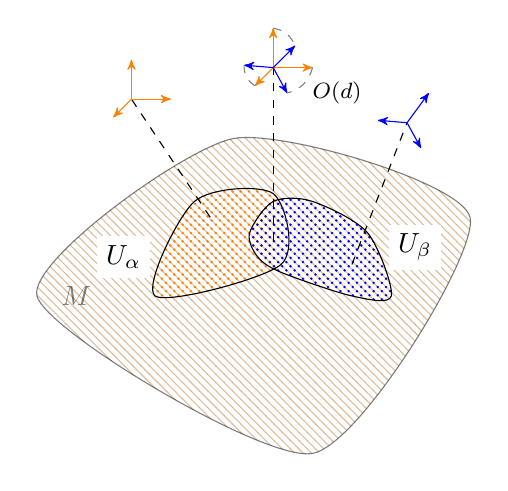
\begin{tikzpicture}

%    % Functions i
%    \path[->] (0.8, 0) edge [bend right] node[left, xshift=-2mm] {$\phi_i$} (-1, -2.9);
%    \draw[white,fill=white] (0.06,-0.57) circle (.15cm);
%    \path[->] (-0.7, -3.05) edge [bend right] node [right, yshift=-3mm] {$\phi^{-1}_i$} (1.093, -0.11);
%    \draw[white, fill=white] (0.95,-1.2) circle (.15cm);
%
%    % Functions j
%    \path[->] (5.8, -2.8) edge [bend left] node[midway, xshift=-5mm, yshift=-3mm] {$\phi^{-1}_j$} (3.8, -0.35);
%    \draw[white, fill=white] (4,-1.1) circle (.15cm);
%    \path[->] (4.2, 0) edge [bend left] node[right, xshift=2mm] {$\phi_j$} (6.2, -2.8);
%    \draw[white, fill=white] (4.54,-0.12) circle (.15cm);

    	% Manifold
	\draw[smooth cycle, tension=0.4, fill=white, pattern color=brown, pattern=north west lines, opacity=0.5] plot coordinates{(2,2) (-0.5,0) (3,-2) (5,1)} node at (0,0) {$M$};

    	% Help lines
    	%\draw[help lines] (-3,-6) grid (8,6);

    	% Subsets
    	\draw[smooth cycle, pattern color=orange, pattern=crosshatch dots] 
        		plot coordinates {(1,0) (1.5, 1.2) (2.5,1.3) (2.6, 0.4)} 
        		node [label={[label distance=-0.3cm, xshift=-2cm, fill=white]:$U_\alpha$}] {};
    	\draw[smooth cycle, pattern color=blue, pattern=crosshatch dots] 
        		plot coordinates {(4, 0) (3.7, 0.8) (3.0, 1.2) (2.5, 1.2) (2.2, 0.8) (2.3, 0.5) (2.6, 0.3) (3.5, 0.0)} 
        		node [label={[label distance=-0.8cm, xshift=.8cm, yshift=1cm, fill=white]:$U_\beta$}] {};
	
	%Frames connections
	\draw[dashed, thin, bend right] (1.7,1) -- (.7,2.5);
	\draw[dashed, thin] (2.5,.7) -- (2.5,2.9);
	\draw[dashed, thin] (3.5,.4) -- (4.2,2.2);
	
	%Frames axis
	\draw[orange, ->] (.7,2.5,0) -- (1.2,2.5,0);
	\draw[orange, ->] (.7,2.5,0) -- (.7,3,0);
	\draw[orange, ->] (.7,2.5,0) -- (.7,2.5,.6); 
	
	\draw[blue, ->] (4.2,2.2,0) -- (4.3,1.8,-.2);
	\draw[blue, ->] (4.2,2.2,0) -- (4.4,2.5,-.2);
	\draw[blue, ->] (4.2,2.2,0) -- (4.1,2.5,.7); 
	
	\draw[orange, ->] (2.5,2.9,0) -- (3,2.9,0);
	\draw[orange, ->] (2.5,2.9,0) -- (2.5,3.4,0);
	\draw[orange, ->] (2.5,2.9,0) -- (2.5,2.9,.6);
	\draw[blue, ->] (2.5,2.9,0) -- (2.6,2.5,-.2);
	\draw[blue, ->] (2.5,2.9,0) -- (2.7,3.1,-.2);
	\draw[blue, ->] (2.5,2.9,0) -- (2.4,3.2,.7); 
	
	\draw[-, dashed, color=gray] (3,2.9,0) to [bend left] (2.6,2.5,-.2) node[right, xshift=+2mm, color= black] {\footnotesize $O(d)$};
	\draw[-, dashed, color=gray] (2.5,3.4,0) to [bend left] (2.7,3.1,-.2);
	\draw[-, dashed, color=gray] (2.5,2.9,.6) to [bend left] (2.4,3.2,.7);
	


%    % First Axis
%    \draw[thick, ->] (-3,-5) -- (0, -5) node [label=above:$\phi_i(U_i)$] {};
%    \draw[thick, ->] (-3,-5) -- (-3, -2) node [label=right:$\mathbb{R}^m$] {};
%
%    % Arrow from i to j
%    \draw[->] (0, -3.85) -- node[midway, above]{$\psi_{ij}$} (4.5, -3.85);
%
%    % Second Axis
%    \draw[thick, ->] (5, -5) -- (8, -5) node [label=above:$\phi_j(U_j)$] {};
%    \draw[thick, ->] (5, -5) -- (5, -2) node [label=right:$\mathbb{R}^m$] {};
%
%    % Sets in R^m
%    \draw[white, pattern color=orange, pattern=crosshatch dots] (-0.67, -3.06) -- +(180:0.8) arc (180:270:0.8);
%    \fill[even odd rule, white] [smooth cycle] plot coordinates{(-2, -4.5) (-2, -3.2) (-0.8, -3.2) (-0.8, -4.5)} (-0.67, -3.06) -- +(180:0.8) arc (180:270:0.8);
%    \draw[smooth cycle] plot coordinates{(-2, -4.5) (-2, -3.2) (-0.8, -3.2) (-0.8, -4.5)};
%    \draw (-1.45, -3.06) arc (180:270:0.8);
%
%    \draw[white, pattern color=blue, pattern=crosshatch dots] (5.7, -3.06) -- +(-90:0.8) arc (-90:0:0.8);
%    \fill[even odd rule, white] [smooth cycle] plot coordinates{(7, -4.5) (7, -3.2) (5.8, -3.2) (5.8, -4.5)} (5.7, -3.06) -- +(-90:0.8) arc (-90:0:0.8);
%    \draw[smooth cycle] plot coordinates{(7, -4.5) (7, -3.2) (5.8, -3.2) (5.8, -4.5)};
%    \draw (5.69, -3.85) arc (-90:0:0.8);
%
\end{tikzpicture}

\end{document}